\let\negmedspace\undefined
\let\negthickspace\undefined
\documentclass[journal]{IEEEtran}
\usepackage[a5paper, margin=10mm, onecolumn]{geometry}
%\usepackage{lmodern} % Ensure lmodern is loaded for pdflatex
\usepackage{tfrupee} % Include tfrupee package

\setlength{\headheight}{1cm} % Set the height of the header box
\setlength{\headsep}{0mm}     % Set the distance between the header box and the top of the text

\usepackage{gvv-book}
\usepackage{gvv}
\usepackage{cite}
\usepackage{amsmath,amssymb,amsfonts,amsthm}
\usepackage{algorithmic}
\usepackage{graphicx}
\usepackage{textcomp}
\usepackage{xcolor}
\usepackage{txfonts}
\usepackage{listings}
\usepackage{enumitem}
\usepackage{mathtools}
\usepackage{gensymb}
\usepackage{comment}
\usepackage[breaklinks=true]{hyperref}
\usepackage{tkz-euclide} 
\usepackage{listings}
% \usepackage{gvv}                                        
\def\inputGnumericTable{}                                 
\usepackage[latin1]{inputenc}                                
\usepackage{color}                                            
\usepackage{array}                                            
\usepackage{longtable}                                       
\usepackage{calc}                                             
\usepackage{multirow}                                         
\usepackage{hhline}                                           
\usepackage{ifthen}                                           
\usepackage{lscape}
\begin{document}

\bibliographystyle{IEEEtran}
\vspace{3cm}

\title{NCERT 12.8.3.1.1}
\author{EE24BTECH11057 - Shivam Shilvant}
% \maketitle
% \newpage
% \bigskip
{\let\newpage\relax\maketitle}

\renewcommand{\thefigure}{\theenumi}
\renewcommand{\thetable}{\theenumi}
\setlength{\intextsep}{10pt} % Space between text and floats

\parindent 0px\textbf{Question:} Find the area of the region bounded by the curve $y=x^2$ and lines $x=1$ , $x=2$ and $x$ axis.

\solution\\
\textbf{Therotical logic:}
\begin{enumerate}
    \item Set up the integral: \\
    The area under the curve can be calculated as:
    \begin{align}
          \text{Area}=\int_{a}^{b}f(x)dx
    \end{align}
    Here:
    \begin{align}
    f(x) = x^2, \quad x_1 = 1, \quad x_2 = 2
    \end{align}
    Thus, the integral becomes:
    \begin{align}
    \text{Area} = \int_{1}^{2} x^2 \, dx
    \end{align}
    \item Compute the integral: \\
    The integral of $x^2$ is:
    \begin{align}
    \int x^2 \, dx = \frac{x^3}{3}
    \end{align}
    \item Evaluate the definite integral: \\
    Substitute the limits of integration:
    \begin{align}
    \text{Area} = \sbrak{\frac{x^3}{3}}_1^2
    \end{align}
    First, calculate $\frac{x^3}{3}$ at $x=2$:
    \begin{align}
    \frac{2^3}{3} = \frac{8}{3}
    \end{align}
    Next, calculate $\frac{x^3}{3}$ at $x=1$:
    \begin{align}
    \frac{1^3}{3} = \frac{1}{3}
    \end{align}
    Subtract the two results:
    \begin{align}
    \text{Area} = \frac{8}{3} - \frac{1}{3} = \frac{7}{3}
    \end{align}

    \item Final result: \\
    area of the region bounded by the curve $y=x^2$ and lines $x=1$ , $x=2$ and $x$ axis is:    \begin{align}
    \frac{7}{3}\text{square units i.e. } 2.3333333333461046
\text{ square units}
    \end{align}
    
\textbf{Computational Logic:} 
Using the trapezoidal rule to get the area. The trapezoidal rule is as follows.
\begin{align}
    \int^{b}_{a} f\brak{x}dx\approx \sum^{N}_{k=1}\frac{f\brak{x_{k+1}}+f\brak{x_{k}}}{2}h
\end{align}
where
\begin{align}
    h=\frac{b-a}{N}
\end{align}
$\therefore$The difference equation obtained is\\
\begin{align}
    A &= \int_a^b f\brak{x}\, dx \approx h\brak{\frac{1}{2}f\brak{a} + f\brak{x_1} + f\brak{x_2} \cdots + f\brak{x_{n-1}} + \frac{1}{2}f\brak{b}}\\
    h &= \frac{b-a}{n}\\
    A &= j_n, \text{ where, } j_{i + 1} = j_i + h\frac{f\brak{x_{i+1}} + f\brak{x_i}}{2}\\ 
        \xrightarrow{} j_{i + 1} &= j_i + h\brak{{x_{i+1}^2}+{x_{i}^2}}\\
    x_{i+1} &= x_i + h\\
    h&=0.00001\\
    n&=300000
\end{align}
Using the code answer obtained is 2.3333333333461046

\begin{figure}[h]
    \centering
    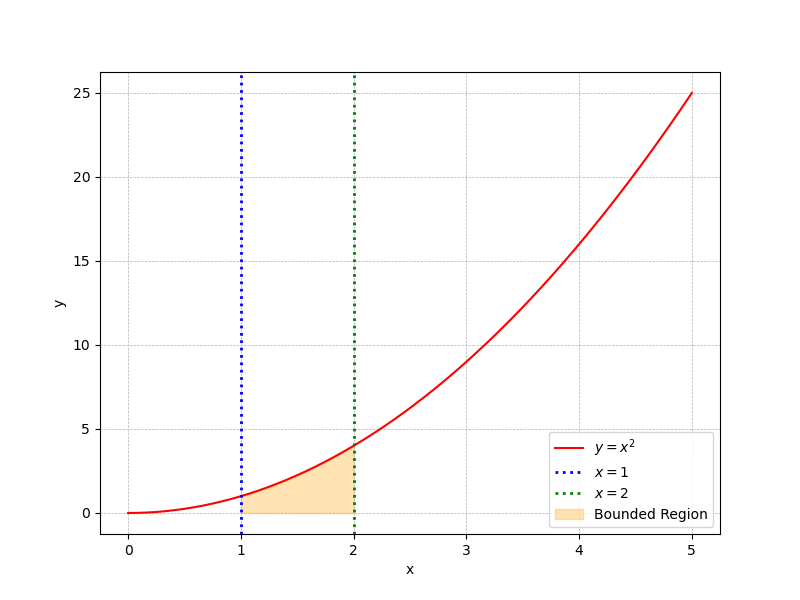
\includegraphics[width=\columnwidth]{figs/fig.png}
 \end{figure}

\end{enumerate}

\end{document}
